% ============================================================================
%
%   TESSERA V1.7
%   ----------------------------------------------------------------------------
%   REAL TELEMETRY TRANSFER ARCHITECTURE
%
%   VERSION
%   -------
%   v1.7 -- Real Telemetry Transfer Architecture · Additive Seal
%          Real-Stream Benchmark Transfer, Dataset Manifests, Leakage Guards,
%          Cross-Regime Replay, No-Repair/Wrong-Repair/Targeted-Repair Ablation,
%          Transfer-Certified Memory, Drift and Staleness Tests, Baseline
%          Regression Guards, Transfer Wound Taxonomy, and Claim-Ceiling Control
%
%   AUTHOR
%   ------
%   James Paul Jackson
%   X / Twitter: @unifiedenergy11
%
%   SOURCE / AUTHOR ATTRIBUTION
%   ---------------------------
%   This document is an additive evolution derived from:
%
%       - TESSERA v1.0: sparse routing, Delta-Phi residuals, evidence gates,
%         alignment certificates, wound ledger, and benchmark locks.
%       - TESSERA v1.1: signal calibration, proxy repair, warning/block/memory
%         separation, wound taxonomy, and durable-memory horizon preservation.
%       - TESSERA v1.2: triadic selective preservation, memory selectivity,
%         phase-window discovery, and triadic non-collapse.
%       - TESSERA v1.3: spectral triadic field architecture, graph/operator
%         declaration, calibrated coherence manifold, governance harm, and
%         certificate-bound selective preservation.
%       - TESSERA v1.4: compressive field memory, sparse graph codec,
%         reconstruction/prediction fidelity, rate-distortion governance,
%         code drift, triadic compression control, and compressed-memory
%         certificates.
%       - TESSERA v1.5: rate-distortion triadic memory, replay validation,
%         false-memory control, codec baselines, and benchmarked compression
%         capability.
%       - TESSERA v1.6: replay-guided codec repair, wound-driven repair,
%         shadow codecs, regression guards, stale-codec detection, and codec
%         lineage hashing.
%
%   DATE
%   ----
%   June 2026
%
%   STATUS
%   ------
%   ADDITIVE TRANSFER AND BENCHMARK PATCH --
%   NOT A CLAIM OF AGI · NOT A CLAIM OF CONSCIOUSNESS · NOT PROOF THAT REAL
%   TELEMETRY SUCCESS GENERALIZES · NOT PERMISSION TO TUNE ON TEST LABELS · NOT
%   PERMISSION TO CLAIM TRANSFER FROM SYNTHETIC DATA ALONE · NOT PROOF THAT
%   REPLAY IS SAFETY · NOT PROOF THAT A REPAIR THAT WORKS ON ONE DATASET WORKS
%   ON ANOTHER · NOT PERMISSION TO BYPASS DATASET MANIFESTS, LEAKAGE GUARDS,
%   BASELINES, REPLAY, VALIDATION, OR CERTIFICATE-BOUND MEMORY
%
%   PURPOSE
%   -------
%   Convert TESSERA v1.6's bounded repair architecture into a real-telemetry
%   transfer protocol:
%
%       Can replay-guided codec repair improve compressed memory on held-out
%       real streams without label leakage, baseline regression, false-memory
%       increase, or stale-codec promotion?
%
%   WHAT THIS IS
%   ------------
%   - A TESSERA v1.7 theory and benchmark-architecture document
%   - A real-telemetry transfer layer for the TESSERA memory/repair stack
%   - A dataset manifest and leakage-control protocol
%   - A cross-regime replay and transfer certificate system
%   - A no-repair, wrong-repair, and targeted-repair ablation plan
%   - A claim-ceiling layer for dataset-specific transfer results
%
%   WHAT THIS IS NOT
%   ----------------
%   - Not proof of general anomaly-detection superiority
%   - Not proof that synthetic performance transfers to real systems
%   - Not permission to tune thresholds on held-out test labels
%   - Not proof that one dataset proves all telemetry domains
%   - Not permission to promote repairs that regress against simple baselines
%   - Not permission for automatic live codec replacement
%
%   EXECUTABLE ANCHOR BLOCK (TESSERA v1.7)
%   --------------------------------------
%   A valid TESSERA v1.7 implementation must:
%
%       (1) preserve the v1.0-v1.6 non-claim locks,
%       (2) preserve spectral routing declarations and codec lineage records,
%       (3) declare dataset manifests, versions, hashes, splits, label access,
%           preprocessing, and leakage controls,
%       (4) separate calibration, training, validation, replay, and final-test
%           windows,
%       (5) compare no-repair, wrong-target repair, generic retraining, and
%           targeted wound-repair under matched budgets,
%       (6) compare against PCA, random projection, autoencoder, reservoir/ESN,
%           persistence, and other declared baselines,
%       (7) report rate-distortion, prediction, replay pass, false-memory,
%           memory selectivity, governance harm, latency, and parameter metrics,
%       (8) block transfer claims when labels leak, calibration is stale, or
%           baselines regress,
%       (9) issue transfer certificates only for dataset-specific results,
%       (10) require human authorization for live codec replacement,
%       (11) and reject any claim that real-stream transfer proves intelligence,
%            safety, truth, alignment, or universal capability.
%
%   CANONICAL LOCK (TESSERA v1.7)
%   -----------------------------
%   - Synthetic success is not transfer.
%   - Transfer is not generalization until held out and replayed.
%   - A dataset result is not a universal claim.
%   - Labels are evidence, not permission to leak.
%   - Repair must beat no-repair and wrong-repair controls.
%   - Baselines remain the claim ceiling.
%   - Real telemetry memory must remain certificate-bound.
%   - Validation remains the reality boundary.
%
% ============================================================================

\documentclass[12pt]{article}

\usepackage[utf8]{inputenc}
\usepackage[T1]{fontenc}
\usepackage[margin=1in]{geometry}
\usepackage{amsmath,amssymb,amsfonts,amsthm}
\usepackage{booktabs,longtable,array}
\usepackage{hyperref}
\usepackage{listings}
\usepackage{xcolor}
\usepackage{tikz}
\usetikzlibrary{arrows.meta,positioning,shapes.geometric,fit,calc}

\newtheorem{definition}{Definition}
\newtheorem{rulebox}{Rule}
\newtheorem{requirement}{Requirement}
\newtheorem{proposition}{Proposition}
\newtheorem{hypothesis}{Hypothesis}
\newtheorem{conjecture}{Conjecture}
\newtheorem{remark}{Remark}
\newtheorem{corollary}{Corollary}

\lstset{basicstyle=\ttfamily\small, breaklines=true, frame=single, columns=fullflexible}

\title{\textbf{TESSERA V1.7}\\
\large Real Telemetry Transfer Architecture}
\author{\textbf{James Paul Jackson}\\[4pt]
\small Tesseract-Efficient Sensory System for Evidence-Routed Alignment\\
\small \texttt{@unifiedenergy11}}
\date{June 2026}

\begin{document}
\maketitle

\begin{abstract}
TESSERA v1.7 is an additive transfer-layer evolution of the replay-guided codec
repair architecture. TESSERA v1.6 established a bounded repair loop: failed
compressed-memory candidates become typed wounds, repair occurs only in shadow
codecs, and durable codec replacement requires replay improvement, baseline
non-regression, false-memory non-increase, certificates, and human
authorization. v1.7 moves that architecture from synthetic pressure tests toward
real telemetry transfer. The system must now prove that compressed memory and
wound-guided repair survive held-out streams, dataset manifests, leakage guards,
real replay windows, and baseline controls. The central claim remains bounded:
real telemetry success is dataset-specific evidence, not a universal claim of
intelligence, safety, or general superiority.
\end{abstract}

%----------------------------------------------------------------------------
\section{Version Relation}
%----------------------------------------------------------------------------

TESSERA v1.7 preserves v1.0 through v1.6 and adds real-telemetry transfer:

\[
\boxed{
TESSERA_{v1.7}
=
TESSERA_{v1.6}
\cup
\{\mathcal{D}_{manifest},\mathcal{L}_{leak},\mathcal{T}_{split},
\mathcal{R}_{cross},\mathcal{A}_{repair},\mathcal{C}_{transfer},\mathcal{K}_{claim}\}.
}
\]

where:

\[
\mathcal{D}_{manifest}=\text{dataset manifest and hash discipline},
\]

\[
\mathcal{L}_{leak}=\text{label leakage and preprocessing guard},
\]

\[
\mathcal{T}_{split}=\text{calibration/train/validation/replay/test separation},
\]

\[
\mathcal{R}_{cross}=\text{cross-regime replay validation},
\]

\[
\mathcal{A}_{repair}=\text{no-repair/wrong-repair/targeted-repair ablation},
\]

\[
\mathcal{C}_{transfer}=\text{real-telemetry transfer certificate},
\]

\[
\mathcal{K}_{claim}=\text{dataset-bound claim ceiling}.
\]

\begin{longtable}{p{0.17\textwidth}p{0.73\textwidth}}
\toprule
\textbf{Version} & \textbf{Contribution preserved in v1.7} \\
\midrule
v1.0 & Sparse routing, Delta-Phi residuals, evidence gates, alignment certificates, wound ledger, and benchmark locks. \\
v1.1 & Signal calibration, proxy repair, warning/block/memory separation, wound taxonomy, and durable-memory horizon preservation. \\
v1.2 & Triadic selective preservation, memory selectivity, phase-window reasoning, and triadic non-collapse. \\
v1.3 & Spectral routing, graph/operator declaration, calibrated coherence, governance harm, and certificate-bound selective preservation. \\
v1.4 & Compression as capability mechanism: sparse graph codec, reconstruction/prediction fidelity, rate-distortion governance, and compressed-memory certificates. \\
v1.5 & Rate-distortion triadic memory, replay validation, false-memory control, codec baselines, and benchmark discipline. \\
v1.6 & Replay-guided codec repair: wound-driven repairs, shadow codecs, acceptance gates, false-memory demotion, stale-codec detection, and codec lineage hashing. \\
v1.7 & Real telemetry transfer: dataset manifests, leakage guards, split discipline, cross-regime replay, repair ablations, transfer certificates, and claim ceilings. \\
\bottomrule
\end{longtable}

\begin{remark}
TESSERA v1.7 is not a larger claim. It is a harder test. It asks whether the
memory and repair architecture remains useful when synthetic convenience is
removed and real streams impose drift, imbalance, stale calibration, partial
labels, and baseline pressure.
\end{remark}

%----------------------------------------------------------------------------
\section{Non-Claim Lock}
%----------------------------------------------------------------------------

\begin{rulebox}[v1.7 Non-Claim Lock]
TESSERA v1.7 does not claim that real telemetry transfer proves general
intelligence, general anomaly-detection superiority, biological validity,
safety, truth, or alignment. A real-stream result is scoped evidence for a
declared dataset, split, metric bundle, baseline set, and transfer certificate.
Validation remains the reality boundary.
\end{rulebox}

Therefore:

\[
\operatorname{SyntheticWin}\not\Rightarrow\operatorname{RealTransfer}.
\]

\[
\operatorname{DatasetWin}\not\Rightarrow\operatorname{UniversalClaim}.
\]

\[
\operatorname{ReplayPass}\not\Rightarrow\operatorname{Safety}.
\]

\[
\operatorname{TargetedRepairWin}\not\Rightarrow\operatorname{UnboundedSelfModification}.
\]

\[
\operatorname{LabelAccess}\not\Rightarrow\operatorname{TuningPermission}.
\]

\[
\operatorname{BaselineRegression}=1\Rightarrow\operatorname{ClaimCeilingLowered}.
\]

%----------------------------------------------------------------------------
\section{Core Thesis}
%----------------------------------------------------------------------------

The v1.7 thesis is:

\begin{center}
\fbox{\begin{minipage}{0.92\textwidth}
A TESSERA memory or codec-repair claim transfers to real telemetry only if it
survives dataset manifests, leakage guards, held-out replay, no-repair and
wrong-repair controls, baseline non-regression, false-memory non-increase, and a
transfer certificate.
\end{minipage}}
\end{center}

The compact law is:

\[
\boxed{
TransferClaim
=
\mathbf{1}[G_{dataset}\wedge G_{leak}\wedge G_{split}\wedge G_{replay}
\wedge G_{repairAblation}\wedge G_{baseline}\wedge G_{falseMem}\wedge G_{cert}].
}
\]

where:

\[
G_{dataset}=\text{manifested dataset and hash record},
\]

\[
G_{leak}=\text{no leakage from labels, future windows, or test statistics},
\]

\[
G_{split}=\text{separate calibration, train, validation, replay, and final test},
\]

\[
G_{replay}=\text{held-out replay pass},
\]

\[
G_{repairAblation}=\text{targeted repair beats no-repair and wrong-repair controls},
\]

\[
G_{baseline}=\text{no regression against declared baselines},
\]

\[
G_{falseMem}=\text{false-memory rate remains bounded},
\]

\[
G_{cert}=\text{transfer certificate passes}.
\]

%----------------------------------------------------------------------------
\section{Dataset Manifest}
%----------------------------------------------------------------------------

\begin{definition}[Dataset Manifest]
A dataset manifest is the evidence record that makes a real-telemetry result
reconstructable, bounded, and auditable.
\end{definition}

A valid manifest stores:

\[
\mathcal{D}_{manifest}=\{name,source,version,hash,channels,timebase,labels,
preprocess,splitPolicy,license,knownCaveats\}.
\]

Candidate benchmark families may include real-time anomaly streams, spacecraft
telemetry, industrial/cyber-physical telemetry, and time-series anomaly archives.
They must be treated as candidate evidence surfaces, not as universal proof.

\begin{rulebox}[Manifest Before Metric Rule]
No real-telemetry metric may be promoted unless the dataset manifest, split
hashes, preprocessing recipe, and label-access policy are recorded first.
\end{rulebox}

\begin{lstlisting}
{
  "schema": "TESSERA-v1.7-dataset-manifest",
  "dataset_name": "NAB|SMAP|MSL|SWaT|UCR|custom",
  "dataset_version": "declared-version-or-commit",
  "raw_data_hash": "sha256:...",
  "preprocess_hash": "sha256:...",
  "label_policy": "hidden_until_final|validation_only|unlabeled|synthetic_labels",
  "time_order_preserved": true,
  "split_policy": {
    "calibration": "time range/hash",
    "train": "time range/hash",
    "validation": "time range/hash",
    "replay": "time range/hash",
    "final_test": "time range/hash"
  },
  "leakage_controls": {
    "future_statistics_blocked": true,
    "test_labels_blocked_from_tuning": true,
    "preprocessing_fit_on_train_only": true
  },
  "known_caveats": []
}
\end{lstlisting}

%----------------------------------------------------------------------------
\section{Leakage Guard}
%----------------------------------------------------------------------------

\begin{definition}[Telemetry Leakage]
Telemetry leakage occurs when future windows, held-out labels, test statistics,
or validation-derived thresholds influence calibration, training, repair, or
promotion decisions.
\end{definition}

Leakage invalidates transfer claims:

\[
Leakage=1\Rightarrow TransferClaim=0.
\]

Common leakage channels:

\begin{longtable}{p{0.28\textwidth}p{0.62\textwidth}}
\toprule
\textbf{Leakage channel} & \textbf{Control} \\
\midrule
Future normalization statistics & fit scalers only on calibration/train windows. \\
Test labels & no threshold tuning or repair routing from final-test labels. \\
Window overlap & prevent same event from appearing in train and test windows. \\
Replay contamination & replay set must be held out from repair fitting. \\
Anomaly-aware preprocessing & preprocessing cannot use anomaly labels unless declared as supervised validation. \\
Repeated hyperparameter tuning & final-test access must be single-pass or ledgered with claim downgrade. \\
\bottomrule
\end{longtable}

\begin{rulebox}[No Hidden Label Rule]
If labels influence threshold selection, repair routing, or codec promotion,
that influence must be declared. Hidden label influence invalidates the claim.
\end{rulebox}

%----------------------------------------------------------------------------
\section{Split Discipline}
%----------------------------------------------------------------------------

TESSERA v1.7 separates five windows:

\[
\mathcal{T}_{split}=\{W_{cal},W_{train},W_{val},W_{replay},W_{test}\}.
\]

\begin{longtable}{p{0.16\textwidth}p{0.74\textwidth}}
\toprule
\textbf{Window} & \textbf{Purpose} \\
\midrule
$W_{cal}$ & estimate amplitude bands, normalization, spectral/coherence ranges, and codec freshness baseline. \\
$W_{train}$ & fit encoder/decoder/predictor or non-parametric codec components. \\
$W_{val}$ & select thresholds, code budgets, and repair policy without touching final test. \\
$W_{replay}$ & retest candidates and shadow repairs after delay or perturbation. \\
$W_{test}$ & final held-out transfer estimate; no repair or threshold tuning allowed. \\
\bottomrule
\end{longtable}

\begin{rulebox}[Final Test Boundary]
The final test window may produce evidence, not tuning. Any tuning after final
test access creates a new experiment and lowers or resets the claim ceiling.
\end{rulebox}

%----------------------------------------------------------------------------
\section{Real-Telemetry Transfer Ladder}
%----------------------------------------------------------------------------

\begin{definition}[Transfer State Ladder]
The transfer ladder prevents synthetic or validation-only evidence from being
presented as real-telemetry transfer.
\end{definition}

\[
\mathcal{L}_{transfer}=\{T_0,T_1,T_2,T_3,T_4,T_5\}.
\]

\begin{longtable}{p{0.12\textwidth}p{0.23\textwidth}p{0.55\textwidth}}
\toprule
\textbf{Level} & \textbf{Name} & \textbf{Meaning} \\
\midrule
$T_0$ & Synthetic & result exists only on generated streams. \\
$T_1$ & Real-calibrated & real data manifest and calibration window exist. \\
$T_2$ & Real-candidate & codec/gate candidate passes validation windows. \\
$T_3$ & Replay-surviving & candidate or repair passes held-out replay. \\
$T_4$ & Baseline-surviving & result survives declared baselines and ablations. \\
$T_5$ & Transfer-certified & final test, certificate, claim ceiling, and lineage all pass. \\
\bottomrule
\end{longtable}

\begin{rulebox}[No Transfer Level Skipping]
A result may not move from synthetic or validation-only evidence directly to a
transfer claim. Dataset manifest, replay survival, baseline survival, and final
test certificate are required.
\end{rulebox}

%----------------------------------------------------------------------------
\section{Repair Ablation Protocol}
%----------------------------------------------------------------------------

The key V1.7 test is not simply whether repair helps. It is whether typed
wound-targeted repair helps more than weaker controls.

\[
\mathcal{A}_{repair}=\{NoRepair,RandomRepair,WrongTargetRepair,GenericRetrain,TargetedWoundRepair\}.
\]

\begin{longtable}{p{0.24\textwidth}p{0.66\textwidth}}
\toprule
\textbf{Ablation} & \textbf{Purpose} \\
\midrule
NoRepair & measures natural performance without codec adaptation. \\
RandomRepair & checks whether any perturbation appears to help by chance. \\
WrongTargetRepair & checks whether wound routing matters. \\
GenericRetrain & tests ordinary retraining pressure without typed wound routing. \\
TargetedWoundRepair & tests the TESSERA v1.6 repair thesis. \\
\bottomrule
\end{longtable}

Targeted repair is supported only if:

\[
\boxed{
U^{targeted}_{transfer}>
\max(U^{no},U^{random},U^{wrong},U^{generic})+\epsilon_T
}
\]

while:

\[
R^{targeted}_{falseMem}\leq R^{old}_{falseMem}+\epsilon_F,
\]

\[
H^{targeted}_{gov}\leq H^{old}_{gov}+\epsilon_H.
\]

\begin{rulebox}[Wrong-Repair Control Rule]
A wound-repair claim is weak unless targeted repair beats wrong-target repair.
If wrong repair performs equally well, the wound-routing mechanism is not yet
supported.
\end{rulebox}

%----------------------------------------------------------------------------
\section{Transfer Utility}
%----------------------------------------------------------------------------

Define real-telemetry memory utility:

\[
U^{real}_{mem}=U_{comp}\cdot U_{pred}\cdot \Omega_{\Phi}\cdot \Omega_Z\cdot S_{gov}\cdot G_{cert}.
\]

Replay-adjusted transfer utility:

\[
\boxed{
U_{transfer}=U^{real}_{mem}\cdot Q_{replay}\cdot (1-R_{falseMem})\cdot
(1-H^{replay}_{gov})\cdot G_{baseline}\cdot G_{leak}.
}
\]

Corrected real memory selectivity:

\[
S^{real}_{mem}=P(G_{memory}=1\wedge G_{replay}=1\mid normal)
-P(G_{memory}=1\wedge G_{replay}=1\mid anomaly).
\]

Baseline gap:

\[
BaselineGap=Score_{TESSERA}-\max_{b\in\mathcal{B}}Score_b.
\]

\begin{rulebox}[Baseline Sets the Ceiling]
If TESSERA fails to exceed simple baselines at matched budget, the valid claim
may still discuss observability, certificates, or repair diagnostics, but not
superior transfer capability.
\end{rulebox}

%----------------------------------------------------------------------------
\section{Real-Telemetry Wound Taxonomy}
%----------------------------------------------------------------------------

\[
\begin{aligned}
\mathcal{W}_{v1.7}=\{&W_{leakage},W_{split},W_{labelscarce},W_{drift},W_{regime},
W_{baseline},\\
&W_{transferfail},W_{replaytransfer},W_{staleReal},W_{overfitRepair},
W_{claimceiling}\}.
\end{aligned}
\]

\begin{longtable}{p{0.24\textwidth}p{0.66\textwidth}}
\toprule
\textbf{Wound} & \textbf{Meaning} \\
\midrule
$W_{leakage}$ & label, future-window, preprocessing, or replay leakage detected. \\
$W_{split}$ & invalid or ambiguous calibration/train/validation/replay/test split. \\
$W_{labelscarce}$ & insufficient labels to support the claimed metric or repair route. \\
$W_{drift}$ & distribution shift detected after calibration or repair. \\
$W_{regime}$ & new operating mode not represented in calibration or replay. \\
$W_{baseline}$ & TESSERA underperforms a matched simple baseline. \\
$W_{transferfail}$ & synthetic or validation performance fails on real held-out streams. \\
$W_{replaytransfer}$ & candidate passes validation but fails cross-regime replay. \\
$W_{staleReal}$ & codec is stale under live or real-data distribution. \\
$W_{overfitRepair}$ & repair improves wounds but degrades normal or boundary replay. \\
$W_{claimceiling}$ & evidence supports a narrower claim than the document or public surface states. \\
\bottomrule
\end{longtable}

\begin{rulebox}[Transfer Wound Rule]
A failed transfer is not a failure of the entire architecture. It is a typed
wound that lowers the claim ceiling and routes the next experiment.
\end{rulebox}

%----------------------------------------------------------------------------
\section{Real Telemetry Transfer Certificate}
%----------------------------------------------------------------------------

\begin{lstlisting}
{
  "schema": "TESSERA-v1.7-real-telemetry-transfer-certificate",
  "system": "TESSERA",
  "version": "v1.7",
  "experiment_id": "sha256:...",
  "dataset_manifest_hash": "sha256:...",
  "codec_lineage_hash": "sha256:...",
  "split_hashes": {
    "calibration": "sha256:...",
    "train": "sha256:...",
    "validation": "sha256:...",
    "replay": "sha256:...",
    "final_test": "sha256:..."
  },
  "leakage_guard": {
    "future_statistics_blocked": true,
    "test_labels_used_for_tuning": false,
    "replay_held_out_from_repair": true,
    "status": "pass|fail"
  },
  "ablation_results": {
    "no_repair": {"transfer_utility": 0.0},
    "random_repair": {"transfer_utility": 0.0},
    "wrong_target_repair": {"transfer_utility": 0.0},
    "generic_retrain": {"transfer_utility": 0.0},
    "targeted_wound_repair": {"transfer_utility": 0.0}
  },
  "baseline_results": {
    "pca": {},
    "random_projection": {},
    "autoencoder": {},
    "reservoir": {},
    "persistence": {}
  },
  "tessera_metrics": {
    "U_transfer": 0.0,
    "S_mem_real": 0.0,
    "H_gov_replay": 0.0,
    "false_memory_rate": 0.0,
    "replay_pass_rate": 0.0,
    "baseline_gap": 0.0,
    "latency_ms": 0.0,
    "params": 0
  },
  "claim_ceiling": "diagnostic|dataset_scoped|transfer_supported|rejected",
  "wounds": [],
  "human_authorized": true,
  "certificate_hash": "sha256:..."
}
\end{lstlisting}

\begin{rulebox}[Claim Ceiling Rule]
The transfer certificate must state the strongest permitted claim. Public claims
may not exceed the certificate's claim ceiling.
\end{rulebox}

%----------------------------------------------------------------------------
\section{Algorithm: TESSERA v1.7 Transfer Experiment}
%----------------------------------------------------------------------------

\begin{lstlisting}[language=Python]
def tessera_v17_transfer_experiment(dataset, live_codec, policies):
    # 1. Manifest and split discipline
    manifest = make_dataset_manifest(dataset, policies.split_policy)
    assert manifest.leakage_controls.future_statistics_blocked
    assert not manifest.leakage_controls.test_labels_used_for_tuning

    # 2. Fit calibration and codec only on allowed windows
    calibration = fit_calibration(dataset.calibration_window)
    codec = fit_or_load_codec(live_codec, dataset.train_window, calibration)

    # 3. Run repair ablations on validation/replay windows
    results = {}
    for mode in ["no_repair", "random_repair", "wrong_target_repair",
                 "generic_retrain", "targeted_wound_repair"]:
        shadow = build_shadow_codec(codec, mode, dataset.validation_window)
        repair_cert = evaluate_shadow_repair(
            old_codec=codec,
            shadow_codec=shadow,
            validation=dataset.validation_window,
            replay=dataset.replay_window,
            baselines=policies.baselines,
        )
        results[mode] = repair_cert

    # 4. Select only if targeted repair passes non-regression gates
    selected_codec = select_codec_under_claim_ceiling(codec, results, policies)

    # 5. Final test is read-only evidence generation
    final_metrics = evaluate_final_test(
        codec=selected_codec,
        final_test=dataset.final_test_window,
        baselines=policies.baselines,
        no_tuning=True,
    )

    # 6. Certificate and claim ceiling
    transfer_cert = make_v17_transfer_certificate(
        manifest=manifest,
        ablations=results,
        final_metrics=final_metrics,
        claim_policy=policies.claim_policy,
    )
    return transfer_cert
\end{lstlisting}

%----------------------------------------------------------------------------
\section{Benchmark Program v1.7}
%----------------------------------------------------------------------------

\begin{longtable}{p{0.23\textwidth}p{0.30\textwidth}p{0.37\textwidth}}
\toprule
\textbf{Experiment} & \textbf{Variables} & \textbf{Success criterion} \\
\midrule
Real transfer baseline & dataset, code budget, topology, damping & TESSERA survives simple baselines under matched budget. \\
Repair ablation & no, random, wrong, generic, targeted repair & targeted repair wins without false-memory increase. \\
Leakage stress & with/without leakage guards & leakage detection blocks transfer claim. \\
Replay split stress & replay held-out vs contaminated & contaminated replay is detected or claim downgraded. \\
Regime drift & calibration shift, new mode, off-manifold intervals & stale codec blocks memory and routes repair. \\
Claim ceiling audit & public summary vs certificate & public claim never exceeds certificate. \\
Latency/parameter audit & kernel status and matched baselines & runtime/efficiency claims are separated. \\
\bottomrule
\end{longtable}

Required baselines:

\[
\mathcal{B}_{v1.7}=\{PCA,RandomProjection,DenseAutoencoder,ESN,DenseReservoir,Persistence,EWMA,MatrixProfile\}.
\]

Required metrics:

\[
\begin{aligned}
\mathcal{M}_{v1.7}=\{&U_{transfer},S^{real}_{mem},H^{replay}_{gov},R_{falseMem},Q_{replay},
BaselineGap,\\
&J_{RD},D_{pred},D_{rec},\Delta Z,\Delta\Phi,Latency,Params,StaleRate,ClaimCeiling\}.
\end{aligned}
\]

%----------------------------------------------------------------------------
\section{Updated Linter Rules}
%----------------------------------------------------------------------------

\begin{longtable}{p{0.16\textwidth}p{0.20\textwidth}p{0.54\textwidth}}
\toprule
\textbf{Rule} & \textbf{Tier} & \textbf{Meaning} \\
\midrule
TESSERA701 & Governance & v1.0-v1.6 non-claim locks missing or weakened. \\
TESSERA702 & Data & dataset manifest missing or incomplete. \\
TESSERA703 & Data & raw data hash, split hash, or preprocessing hash missing. \\
TESSERA704 & Leakage & future statistics, labels, or replay windows leaked into tuning. \\
TESSERA705 & Split & calibration/train/validation/replay/test windows fused. \\
TESSERA706 & Repair & targeted repair claimed without no-repair and wrong-repair controls. \\
TESSERA707 & Baseline & transfer claim made despite baseline regression. \\
TESSERA708 & Replay & replay set not held out from repair. \\
TESSERA709 & Memory & false-memory rate increases under transfer. \\
TESSERA710 & Staleness & stale codec permits real-data memory promotion. \\
TESSERA711 & Claim & public claim exceeds transfer certificate ceiling. \\
TESSERA712 & Runtime & speed claim fused with parameter-efficiency claim. \\
TESSERA713 & Generalization & one dataset result presented as universal. \\
TESSERA714 & Authorization & live codec replacement without human authorization. \\
\bottomrule
\end{longtable}

%----------------------------------------------------------------------------
\section{Falsification Surface}
%----------------------------------------------------------------------------

TESSERA v1.7 is weakened or rejected if:

\begin{itemize}
\item real telemetry transfer fails while synthetic success is still claimed as
transfer;
\item leakage is detected in labels, preprocessing, replay, or test statistics;
\item targeted repair fails to beat no-repair, wrong-repair, or generic retrain
controls;
\item simple baselines such as PCA, persistence, or reservoir methods match or
beat TESSERA under the same budget;
\item false-memory rate increases under real streams;
\item stale codec detection fails under regime drift;
\item final-test results are used for threshold or repair tuning;
\item a dataset-scoped result is presented as a universal claim;
\item public claims exceed the transfer certificate ceiling;
\item or live codec replacement bypasses authorization.
\end{itemize}

Compact invalidation rule:

\[
\begin{aligned}
&[TransferClaim\wedge Leakage]
\vee [TransferClaim\wedge \neg DatasetManifest]
\vee [TransferClaim\wedge BaselineRegression]\\
&\vee [RepairClaim\wedge TargetedRepair\leq WrongRepair]
\vee [PublicClaim>ClaimCeiling]\\
&\vee [LiveCodecChange\wedge \neg HumanAuth]
\Rightarrow InvalidTESSERAv1.7Use.
\end{aligned}
\]

%----------------------------------------------------------------------------
\section{Roadmap}
%----------------------------------------------------------------------------

\begin{longtable}{p{0.18\textwidth}p{0.72\textwidth}}
\toprule
\textbf{Version} & \textbf{Purpose} \\
\midrule
v1.7 & Real telemetry transfer: manifests, leakage guards, split discipline,
repair ablations, cross-regime replay, transfer certificates, and claim ceilings. \\
v1.8 & Repository-aware compressed memory: artifact-state compression, route-map
codes, evidence bundles, and software-maintenance replay. \\
v1.9 & Adaptive topology repair: graph rewiring, code-budget repair, spectral
normalization, and topology-lineage certificates under replay constraints. \\
v2.0 & Integrated TESSERA engine: reference implementation, dataset/repair
benchmark suite, report generator, certificate ledger, and claim-ceiling linter. \\
\bottomrule
\end{longtable}

%----------------------------------------------------------------------------
\section{System Diagram}
%----------------------------------------------------------------------------

\begin{center}
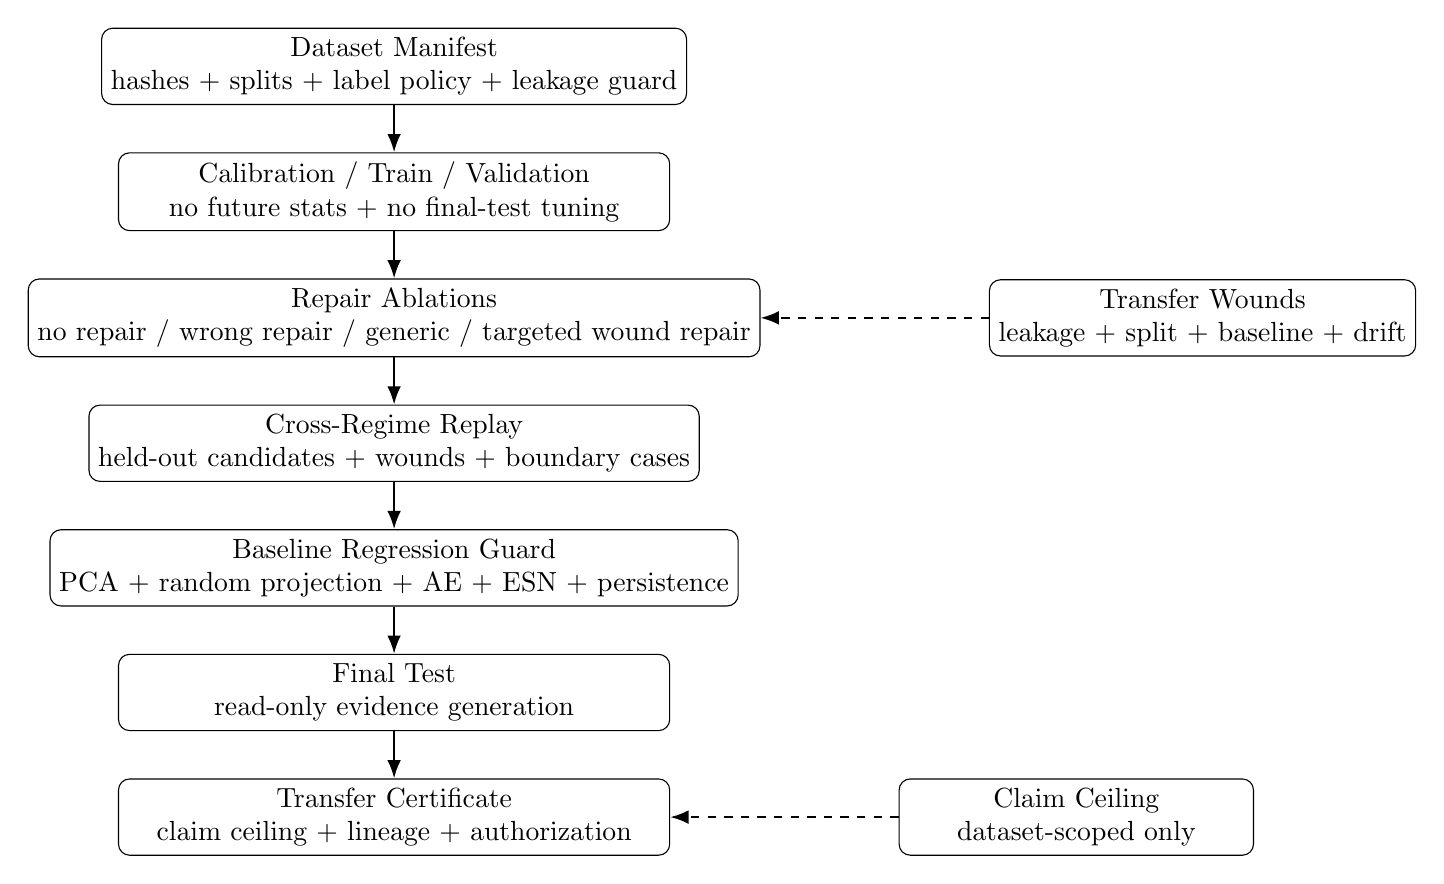
\begin{tikzpicture}[
  node distance=0.60cm,
  box/.style={rectangle, rounded corners, draw, align=center, minimum width=7.0cm, minimum height=0.62cm},
  smallbox/.style={rectangle, rounded corners, draw, align=center, minimum width=4.5cm, minimum height=0.56cm},
  arrow/.style={-Latex, thick}
]

\node[box] (manifest) {Dataset Manifest\\hashes + splits + label policy + leakage guard};
\node[box, below=of manifest] (cal) {Calibration / Train / Validation\\no future stats + no final-test tuning};
\node[box, below=of cal] (repair) {Repair Ablations\\no repair / wrong repair / generic / targeted wound repair};
\node[box, below=of repair] (replay) {Cross-Regime Replay\\held-out candidates + wounds + boundary cases};
\node[box, below=of replay] (base) {Baseline Regression Guard\\PCA + random projection + AE + ESN + persistence};
\node[box, below=of base] (test) {Final Test\\read-only evidence generation};
\node[box, below=of test] (cert) {Transfer Certificate\\claim ceiling + lineage + authorization};

\draw[arrow] (manifest) -- (cal);
\draw[arrow] (cal) -- (repair);
\draw[arrow] (repair) -- (replay);
\draw[arrow] (replay) -- (base);
\draw[arrow] (base) -- (test);
\draw[arrow] (test) -- (cert);

\node[smallbox, right=2.9cm of repair] (wound) {Transfer Wounds\\leakage + split + baseline + drift};
\draw[arrow, dashed] (wound) -- (repair);

\node[smallbox, right=2.9cm of cert] (claim) {Claim Ceiling\\dataset-scoped only};
\draw[arrow, dashed] (claim) -- (cert);

\end{tikzpicture}
\end{center}

%----------------------------------------------------------------------------
\section{Public Framing}
%----------------------------------------------------------------------------

Internal framing:

\begin{center}
\fbox{\begin{minipage}{0.92\textwidth}
TESSERA v1.7 turns real telemetry into the reality boundary for repair. A wound
repair is not transfer until it survives manifests, leakage guards, held-out
replay, baselines, final test, and a transfer certificate.
\end{minipage}}
\end{center}

Public engineering framing:

\begin{center}
\fbox{\begin{minipage}{0.92\textwidth}
TESSERA is a sparse-field memory system that tests compressed memory and repair
on real telemetry through dataset manifests, leakage-safe splits, replay
validation, baseline controls, and dataset-scoped certificates.
\end{minipage}}
\end{center}

Short description:

\begin{center}
\fbox{\begin{minipage}{0.78\textwidth}
Synthetic success is not transfer. Transfer is certificate-bound real-stream
survival.
\end{minipage}}
\end{center}

Required non-claim:

\begin{center}
\fbox{\begin{minipage}{0.78\textwidth}
A dataset win is not a universal claim. Validation remains reality.
\end{minipage}}
\end{center}

%----------------------------------------------------------------------------
\section{Concluding Compression}
%----------------------------------------------------------------------------

TESSERA v1.6 asked:

\begin{center}
\fbox{\begin{minipage}{0.92\textwidth}
How can failed compressed-memory candidates repair the codec without allowing
false memories, stale codecs, or unvalidated updates to compound?
\end{minipage}}
\end{center}

TESSERA v1.7 asks:

\begin{center}
\fbox{\begin{minipage}{0.92\textwidth}
How can that repair architecture survive real telemetry without leakage,
baseline regression, false-memory increase, or claim inflation?
\end{minipage}}
\end{center}

The v1.7 spine is:

\begin{center}
\fbox{\begin{minipage}{0.92\textwidth}
\centering
DatasetManifest $\rightarrow$ LeakageGuard $\rightarrow$ SplitDiscipline
$\rightarrow$ RepairAblation $\rightarrow$ CrossReplay $\rightarrow$ BaselineGuard
$\rightarrow$ FinalTest $\rightarrow$ TransferCertificate.
\end{minipage}}
\end{center}

The transfer law is:

\begin{center}
\fbox{\begin{minipage}{0.92\textwidth}
\centering
TransferClaim $\Rightarrow$ DatasetManifest $\wedge$ LeakageGuard $\wedge$
HeldOutReplay $\wedge$ BaselineNonRegression $\wedge$ ClaimCeiling.
\end{minipage}}
\end{center}

The final lock is:

\begin{center}
\fbox{\begin{minipage}{0.82\textwidth}
\centering
Synthetic success is not transfer. Transfer is certificate-bound real-stream
survival.
\end{minipage}}
\end{center}

Thus TESSERA v1.7 evolves the system from bounded repair into real-telemetry
transfer discipline. The architecture may now test whether its memory and repair
loop survives outside synthetic streams, but every transfer claim is constrained
by dataset manifests, leakage guards, split discipline, ablations, baselines,
held-out replay, final-test evidence, and a certificate-bound claim ceiling.

\end{document}
